\documentclass[conference]{IEEEtran}
\IEEEoverridecommandlockouts
% The preceding line is only needed to identify funding in the first footnote. If that is unneeded, please comment it out.
\usepackage{cite}
\usepackage{amsmath,amssymb,amsfonts}
\usepackage{algorithmic}
\usepackage{graphicx}
\usepackage{textcomp}
\usepackage{xcolor}
\PassOptionsToPackage{hyphens}{url}\usepackage{hyperref}
\usepackage{cleveref}
\usepackage[amssymb]{SIunits}
\def\BibTeX{{\rm B\kern-.05em{\sc i\kern-.025em b}\kern-.08em
    T\kern-.1667em\lower.7ex\hbox{E}\kern-.125emX}}
\begin{document}

\title{Evaluation of HTTP/3 for Media Streaming}

\author{\IEEEauthorblockN{1\textsuperscript{st} Philip Nys}
\IEEEauthorblockA{\textit{Open Distributed Systems} \\
\textit{Technische Universität Berlin}\\
Berlin, Germany \\
p.nys@campus.tu-berlin.de}}


\maketitle

\begin{abstract}
    Media is putting a lot of strain on the internet network and is gaining more and more in popularity. The Transmission Connection Protocol (TCP) has been the defacto protocol for media streaming for well over a decade now, but it has some glaring issues, which hinder the efficiency of media streaming. HTTP/3 was specifically designed to solves them and this document will evaluate several proposed standards for HTTP/3 based media streaming protocols.
\end{abstract}

\begin{IEEEkeywords}
HTTP/3, QUIC, WebTransport, WARP, RUSH, QuicR, MOQT, TCP, UDP, Media Streaming
\end{IEEEkeywords}

\section{Motivation}
In 2017 media streaming has taken up 77\% \cite{b1} of all internet traffic and is expected to have increased this portion to about 82\% at the end of 2022 \cite{b1}. Under normal circumstances this doesn't pose a big issue. However, as the COVID-19 pandemic showed, during early lockdowns where most of the world's population was restricted to stay at home and many of them spent their time streaming media, this could lead to problems. During these lockdowns big content provides like Netfilx \cite{b2}, Amazon Prime Video and YouTube \cite{b3} lowered the bitrate of their content to prevent a crashing of the network.

This requires measures to make the whole media streaming process as efficient as possible while still providing a seamless experience for the viewer.

\section{Current streaming situation}
The current HTTP versions 1.1 and 2 have been well established as defacto media streaming protocols for almost 15 years now, initially with the release of Apple's HTTP Live Streaming (HLS) in 2009 \cite{b4} and later in 2012 in Dynamic Adaptive Streaming over HTTP (DASH) \cite{b5}. These two HTTP versions use the underlying Transmission Control Protocol (TCP), which by nature is a reliable protocol, that means it is guaranteed that the data is arriving not only without errors but also in the correct order. This may seen like a good thing for media streaming, since it is desirable for a to be exactly what TCP guarantees - in the correct order and without errors. However, there are some glaring issues when streaming media using TCP. 

Firstly, TCP has been designed without any encryption or security measures in mind and since well over 80\% of all internet traffic is in fact encrypted \cite{b6} and most of today's media content is subject to encryption, like Digital Rights Management (DRM), it is safe to assume we are always working with encryption, like HTTPS. The problem with this is that initial connection handshakes unnecessarily slow by having to do one TCP handshake and then separately a handshake for the Transport Layer Security (TLS) encryption, which ultimately creates an undesirably high latency, shown in \cref{fig:handshake}.

Secondly, TCP still suffers heavily from Head-of-Line-Blocking (HOL-Blocking). HOL-Blocking occurs on TCP connections when a data packet is delayed, by routing stalls or out of order delivery for example, all the following packets have to wait for the delayed packet for the traffic can flow again \cite{b7}. This can lead to unwanted video buffering or lowered quality by registering a reduced data throughput.

Thirdly, when using TCP the client has to specifically request every individual video segment from the server. This creates a lot of unnecessary internet traffic, since media is split up into small chunks, usually of sizes between 2 and 10 seconds \cite{b8}. Even a small video with a length of 10 minutes can easily have hundreds of segments and big movies can have thousands.

\section{HTTP/3 - What is new?}
To solve the previously stated issues with TCP, a new protocol, QUIC, has been designed to offer an improvement over TCP. 

\subsection{QUIC}
Before TCP was established as state-of-the-art media streaming protocols made use of the unreliable User Datagram Protocol (UDP), protocols like the Real-Time Transport Protocol (RTP) \cite{b9} and Real Time Messaging Protocol (RTMP) \cite{b10} and QUIC comes full circle and again uses UDP as its underlying transport protocol. However, it is a vastly extended form of UDP.

Normally, UDP is an unreliable protocol, which means there is nothing to make sure the data arrives without errors or even arrives at all. QUIC, however, uses UDP to establish so called streams between client and server to send data and also creates additional parallel streams to verify the data has arrived correctly and in case it has not, the data is retransmitted on another parallel stream.

Furthermore, to tackle TCP issues QUIC has been designed with the followed improvements. Firstly, as previously alluded to TLS is optional with TCP, but QUIC mandates to always use TLS. This way it was possible to tightly integrate the TLS handshake along side the opening QUIC handshake. Which reduces the initial connection establishment from two round trip times (twice back and forth from client to server) down to a single round trip time (only once back and forth), as seen in \cref{fig:handshake}.

Secondly, UDP itself does not suffer from HOL-Blocking. However, since QUIC allows sending data on parallel streams, which could cause HOL-Blocking. QUIC has been equipped with sophisticated multiplex algorithms to minimize HOL-Blocking as much as possible.

Thirdly, once a QUIC connection has been established it not only possible for the client to open data streams but also for the server. That means it is entirely possible for the server to push data to client as it sees fit without the client ever having to send out any requests for it. This can completely eliminate the unnecessary requests from the client and reduces the overall traffic when it comes to media streaming. This also makes it possible for the server to start sending the video seg to client as soon as it sends out the connection confirmation to the client. In combination with the sped up opening handshake, this means that the client can receive data right after receiving the connection confirmation from the server, in other words data would be arriving after a single round trip time. Meanwhile, when using TCP and TLS, a client would need to do the TCP handshake, then the TLS handshake, then send  out the first requests and only receive the first data packet after three full round trip times, as depicted in \cref{fig:handshake}.

\subsection{HTTP/3}
HTTP/3 is the most recent version of the Hyper Text Transport Protocol and aims to integrate the QUIC protocol into an HTTP standard \cite{b11}.

\subsection{WebTransport}
WebTransport is an Application Programming Interface (API), which allows a client to connection to an HTTP/3 server and make use of the complete feature set of QUIC. After establishing the WebTransport connection, it enables the client to open unidirectional streams, which only allow the opener (in this case the client) to send data, open bidirectional streams, which allow both peers to send and receive data on this singular stream, receive unidirectional streams opened by the server, on which you can only receive data and receive bidirectional streams opened by the server, as well as sending and receiving datagrams, which are basic unreliable UDP packets \cite{b12}.

\section{Comparison - TCP vs QUIC}
To reiterate the three most important improvements over TCP QUIC brings to the table, let's compare them directly. The first improvement is the lower latency by combining the opening protocol and TLS handshakes into a single handshake. This way using QUIC the client can receive data just shortly after receiving connection confirmation from the server, usually rounded to 1.5RTT (round trip times), compared to the sequential TCP, TLS handshake followed by the request for the first data segment, a full 3RTT in total.

Related to this, when using QUIC the client no longer has to request ever individual data segment one by one, instead the server enabled to push data to the client without it explicitly requesting it.

Finally, with TCP TLS encryption was just an optional feature and would also slow it down when using it, meanwhile, QUIC offers better security by mandating to be always encrypted, while also not trading off security for performance. 

\begin{figure}
    \fbox{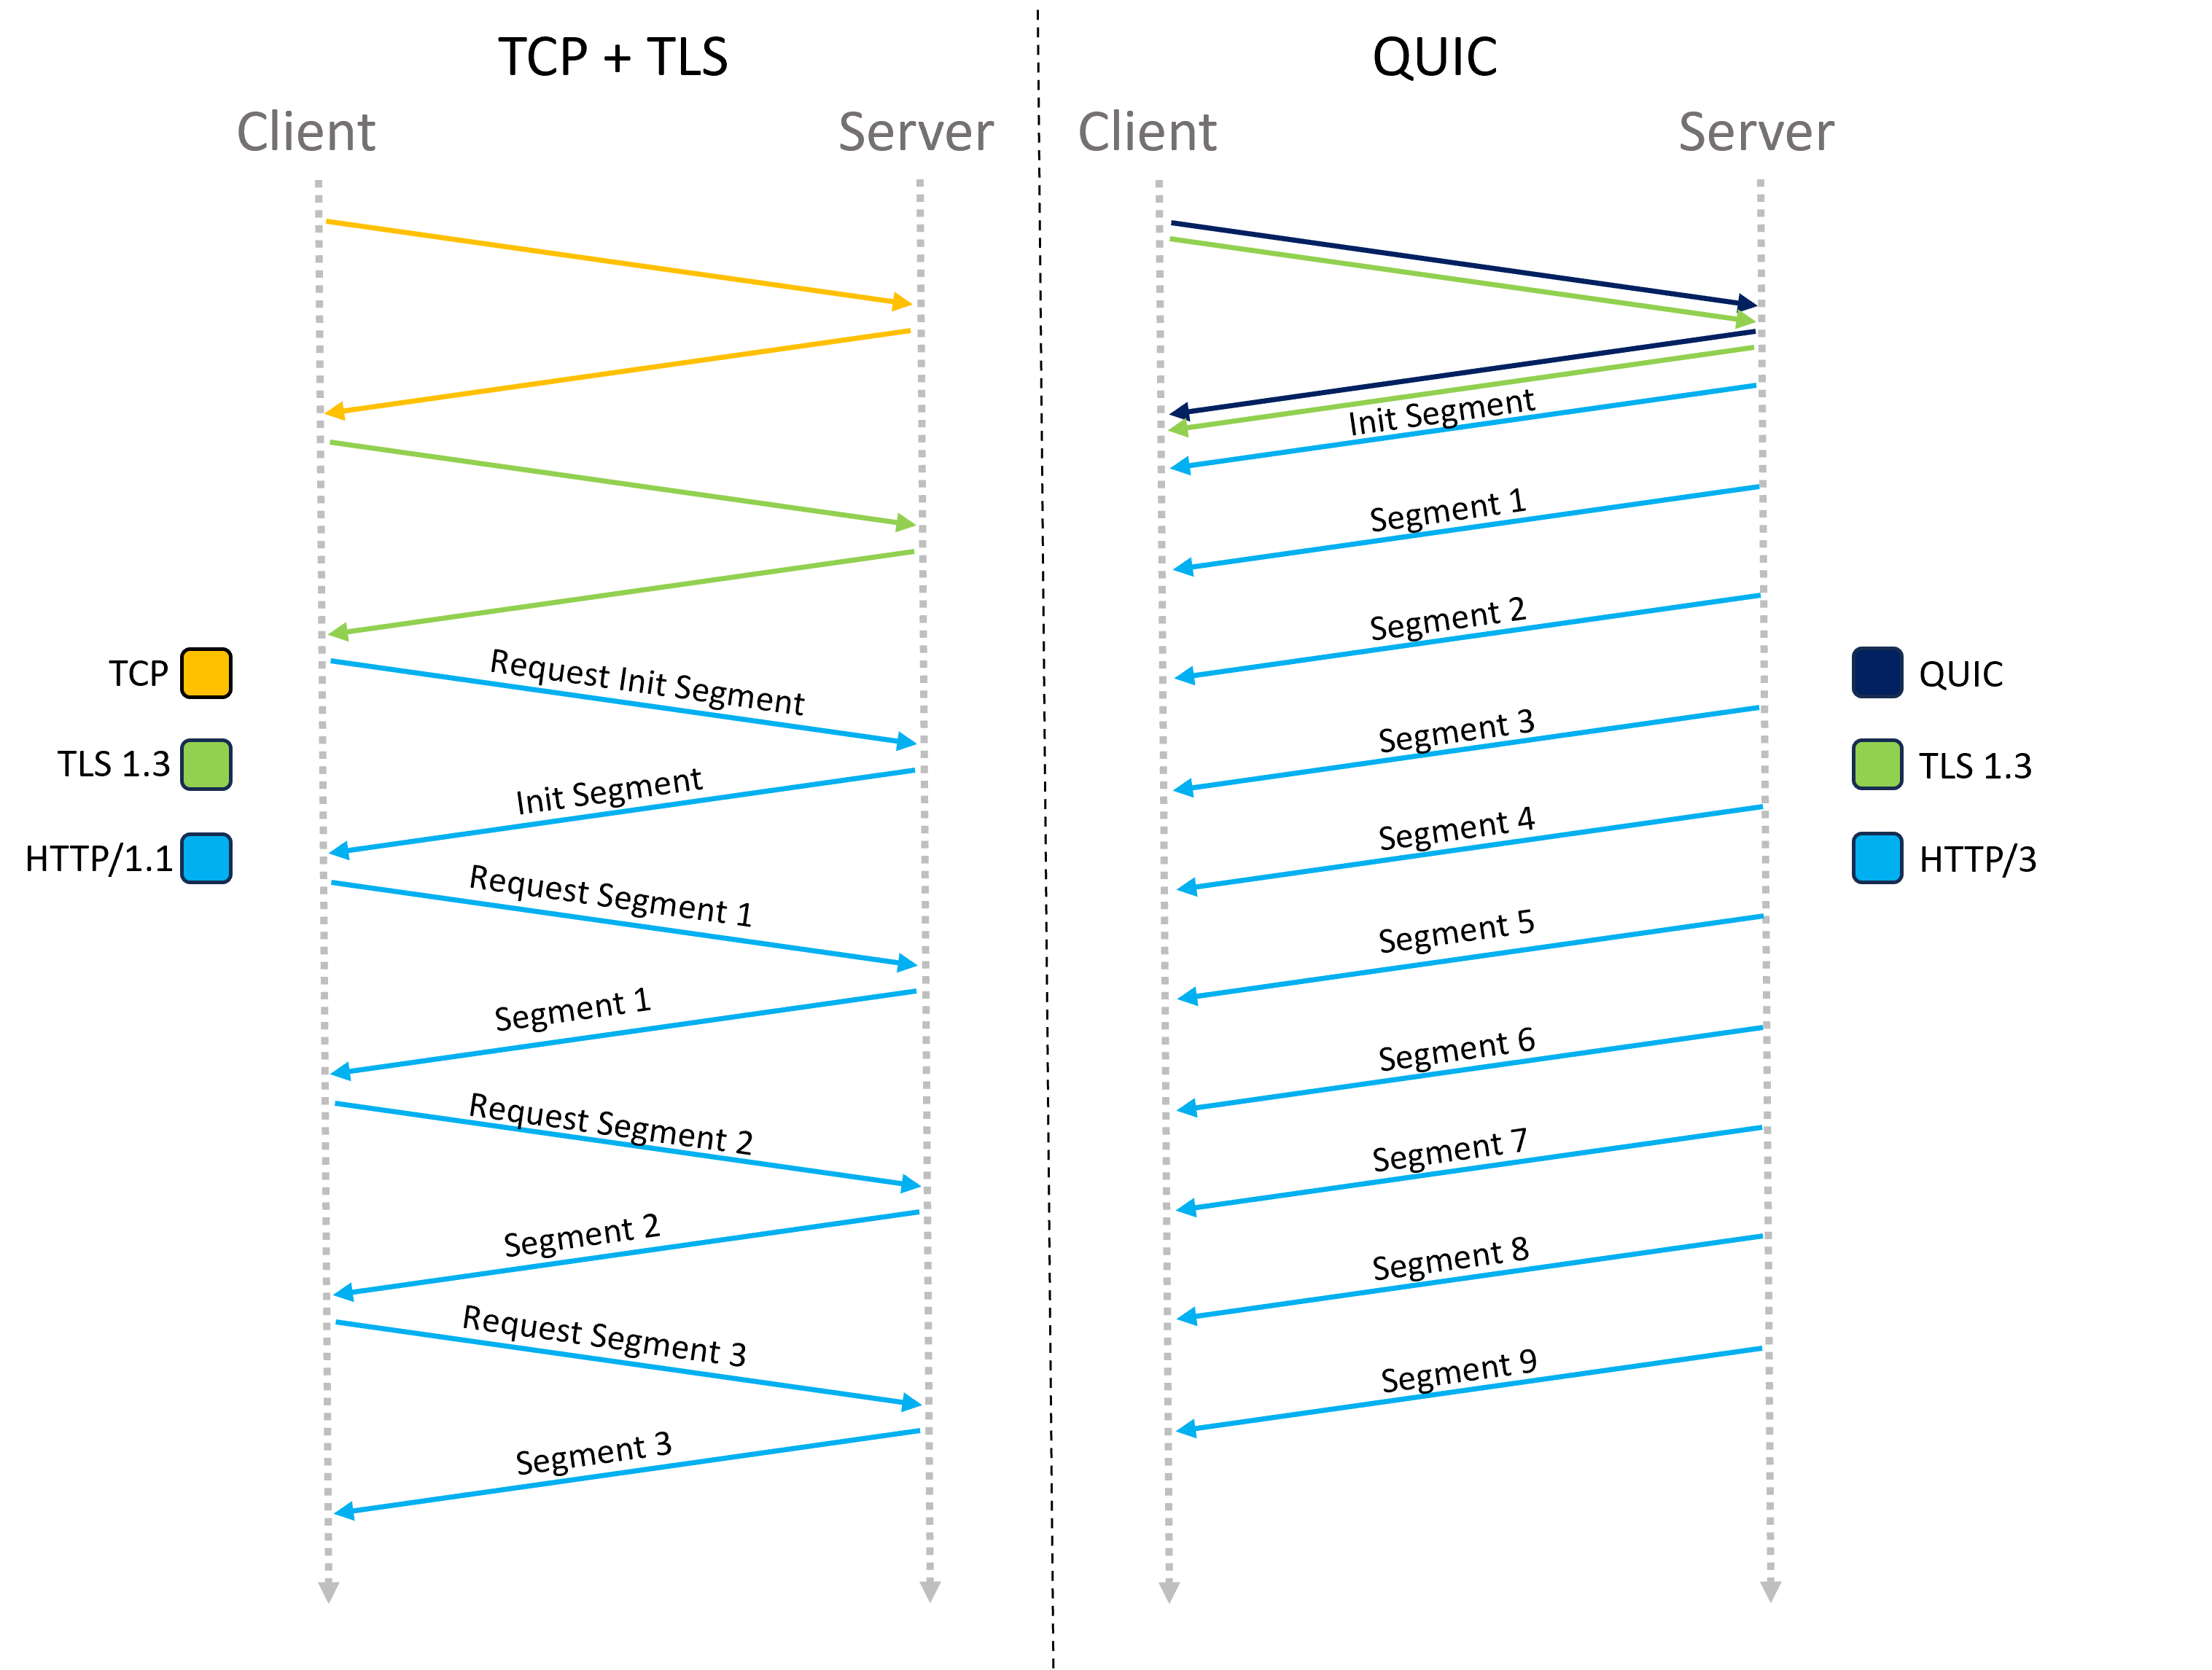
\includegraphics[width=0.49\textwidth]{images/handshake.png}}
    \caption{Comparison - Handshakes of TCP and QUIC}
    \label{fig:handshake}
\end{figure}

\section{Proposed Standards}
In 2021 an Internet Engineering Task Force (IETF) working group Media Over QUIC (moq) has been founded to work on building a standard for streaming media using QUIC. In these years there have been several standards. I have analyzed the code of three of them, set them up on a laptop and will evaluate them.

Please note these propositions are highly experimental were tricky to setup, on my repository for this project \cite{b13} I have provided additional help to make it easier, if you want to see them running for yourself.

\subsection{RUSH}
The first proposition is RUSH (Reliable - unreliable - Streaming Protocol) \cite{b14} by Facebook. RUSH has been designed for real time live streaming.

The server code is written in go using a proprietary version of the $webtransport-go$ package \cite{b15} and the client is a plain JavaScript website. 

This RUSH demo consists of two repositories, one for the clients \cite{b16} and one for the server \cite{b17}. The client side provides one website acting as the content creator (the streamer), as well as a second website which can act as one of the viewer, who watches the stream. The server in this demo is basic relay, which receives the video stream from the streamer and then forwards them to all the viewers subscribed to the stream.

The process of this demo looks the following and as seen in \cref{fig:rush}. The streamer opens the streamer website and starts the stream. Starting the stream will grab hijack the video feed from the connected webcam, open a WebTransport connection to the relay server. The $ID$ is a random string of numbers created on the website and is used on correctly steer the video stream to the correct viewers. The video feed from the server will be piped through a encoder which prepares the data for transmission. The encoded video frames are then transmitted by sending every individual frame on its own WebTransport unidirectional stream to the server. Sending every frame individually ensures that the feed arrives as fast as possible, by keeping packets as small as possible. 

The server is listening on the "\url{/moqingest/:ID}" and "\url{/moqdelivery/:ID}" endpoints, receives the frames on the ingest endpoint and then saves the frames in memory and then relays the frames to every subscribed viewer on the delivery endpoint, again by sending every single frame on its own unidirectional stream.

In the meantime you can open the viewer website and copy the StreamID from the streamer website and paste it on the viewer website and by pressing start you will start receiving the webcam feed from the streamer with minimal latency.

Please note, when running the demo I didn't receive any video output on the viewer client and I was unfortunately unable to resolve this issue in the time frame of this project. All I was able to see were numerous outputs showing statistics and metrics of the current streaming sessions. However, the people behind this demo provided a demo video \cite{b18} which also properly has the relay server running offsite. The server was running in Frankfurt, Germany and both clients were sitting in Barcelona, Spain. In the video they ambitiously configured the player buffer to $10ms$ and audio and video jitter both to $95ms$ and they showed an end-to-end latency (from capturing the webcam feed to displaying the video on the viewer client) of around $300ms$.

\begin{figure}
    \fbox{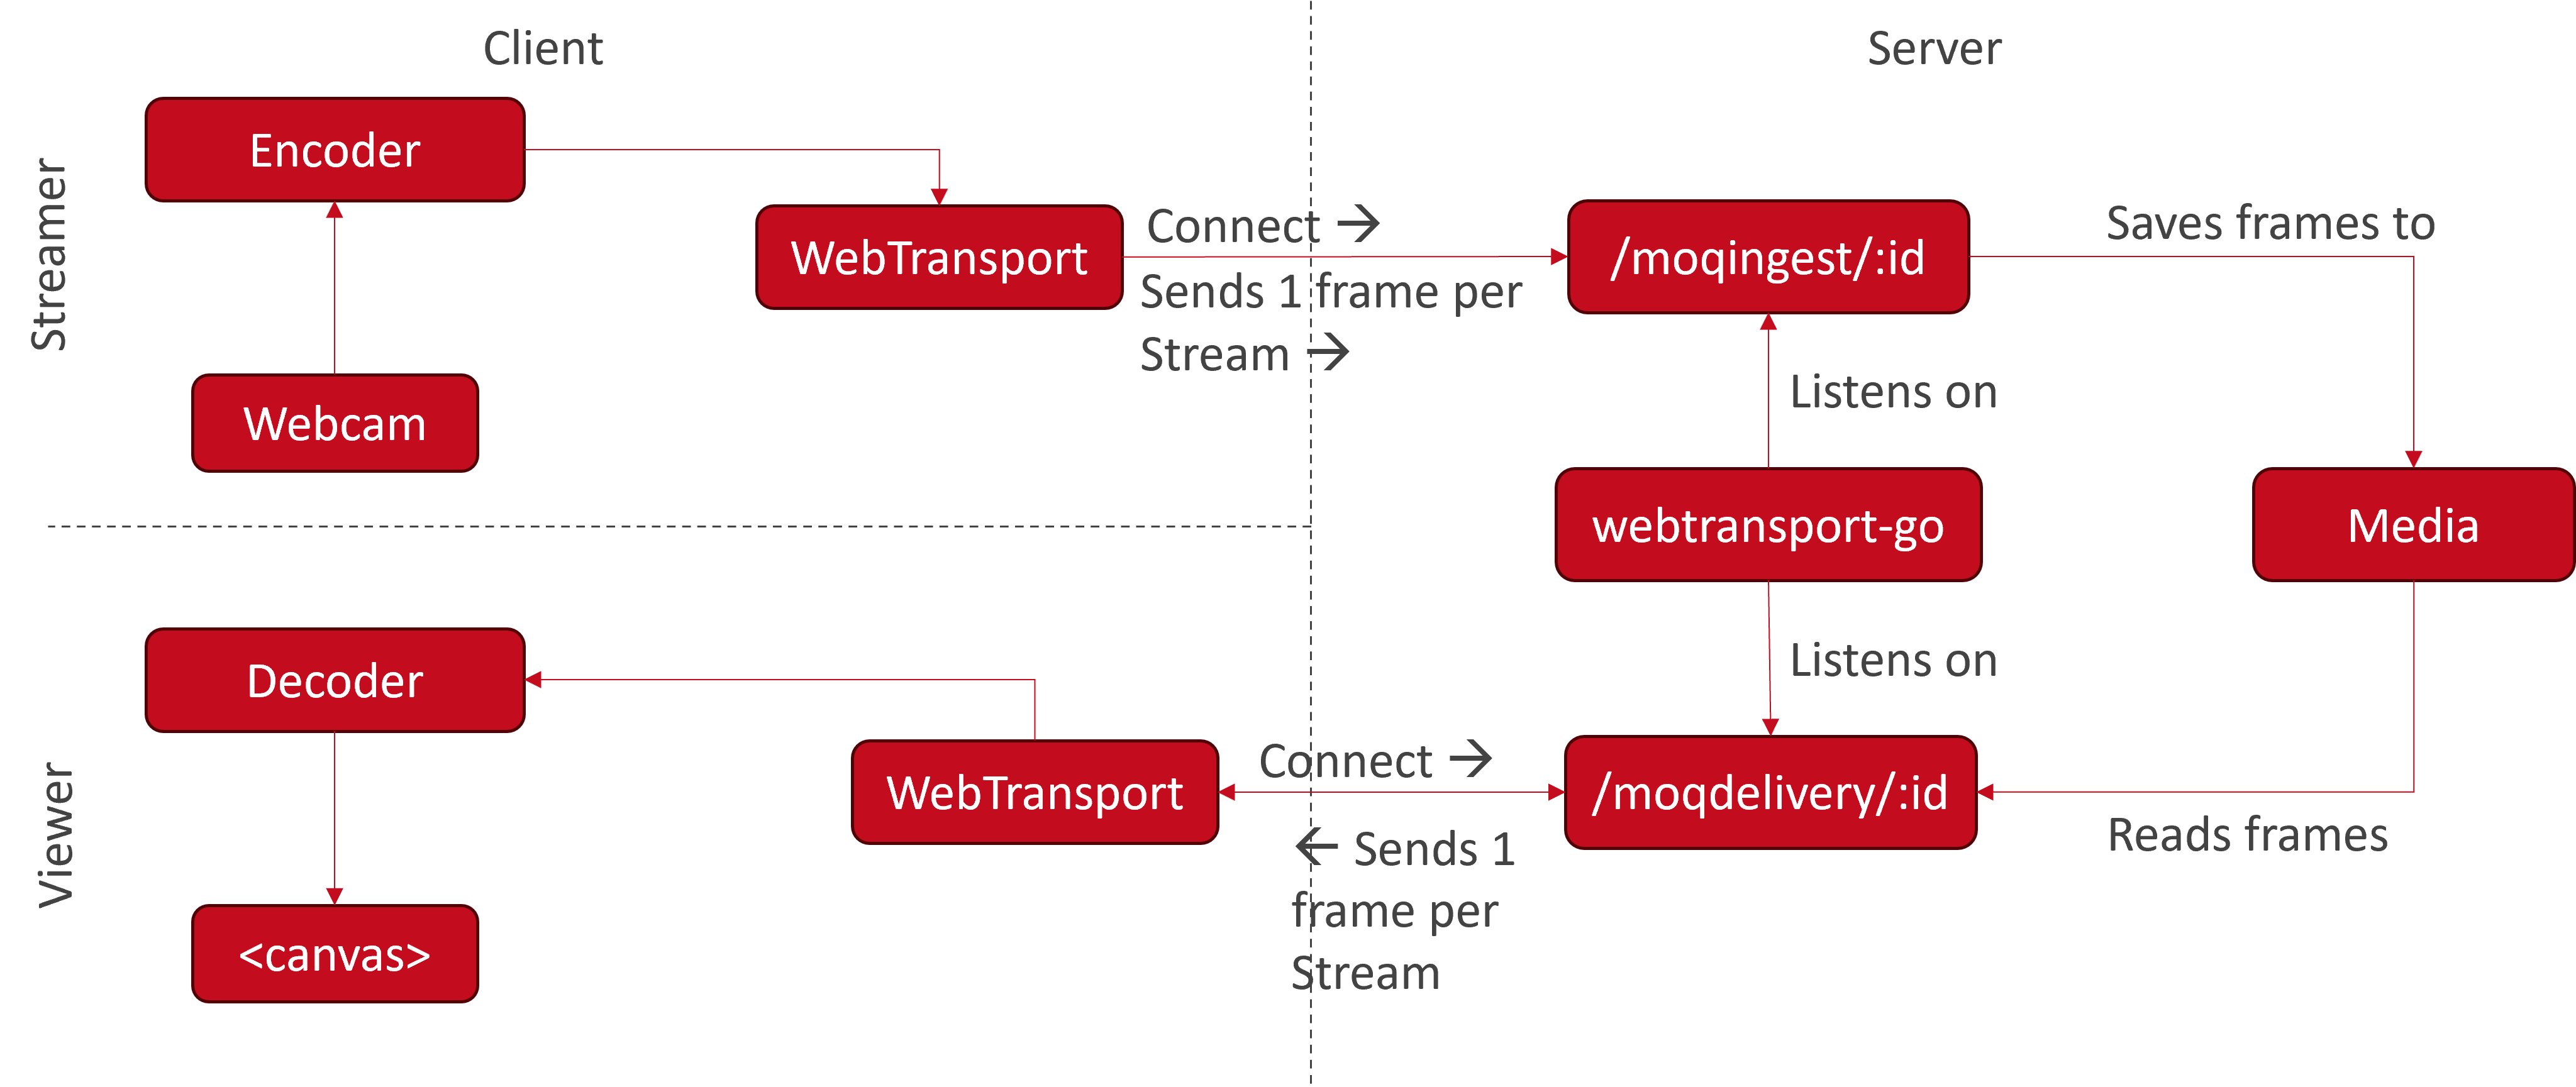
\includegraphics[width=0.49\textwidth]{images/rush.png}}
    \caption{Flow chart RUSH protocol}
    \label{fig:rush}
\end{figure}

\subsection{QuicR}
The second proposition is QuicR by Cisco \cite{b19}. QuicR has been designed to a general transport protocol for a broad range of application at different latency stages, but many for use cases requiring very low latency, for example live streaming, two way video conferencing, multiplayer video games, etc.

The provided demo \cite{b20} was made for macOS with a dedicated swift program acting as clients and the server was written in C++ using the $libquicr$ \cite{b21} API which is an implementation of the $quicrq$ \cite{b22} library.

Personally, I was unable to get the demo running on the provided MacBook, since I kept getting an error when build the project and I am not familiar with macOS to get the issues resolved in the time frame of this project.

Fortunately, the repository provided two demo videos showing the demo in action. The first demo showed an scenario of a two-way video call with the server running on the Akamai Network in Atlanta, USA and both clients sitting in London, UK \cite{b23}. The second demo showed a use case of having a single streamer and (in this case) three viewers watching the streamer. In this demo the server was running on AWS in Ohio, USA and the clients were sitting in San Josè, USA \cite{b24}. In both demo video it can be observed that the latency was barely noticeable.

\subsection{WARP}
The third and final proposition is WARP by Twitch \cite{b25}. WARP has been designed for ultra low latency live streaming.

The server was written in go using a heavily modifier version of the $webtransport-go$ package \cite{b26} and the client is a plain JavaScript website. 

The demo setup consists similarly to RUSH of a server and a client. See \cref{fig:warp} for graphical depiction of the demo. However, in this case the demo is simplified by foregoing the streamer client by simply streaming from a local manifest file. Please note in the code there was a comment specifically noting that this was made just for demo purposes and the intended use is for live streaming. 

The setup in this demo starts with the client connecting to the server using WebTransport and then listening for incoming unidirectional streams. The server meanwhile is listening on the "\url{/watch}" endpoint. Once the connection has been established the server starts loading the video segments from the local manifest and initiates an $Invoker$, which is a custom package that allows running $goroutines$ easily and safely. $Goroutines$ allow the execution of code in parallel in go. This $Invoker$ runs five $goroutines$ in total:

\begin{itemize}
    \item runAccept: accepting bidirectional streams
    \item runAcceptUni: accepting unidirectional streams
    \item runInit: opening a new stream and sending the init segments
    \item runAudio: infinite loop, sending all audio segments
    \item runVideo: infinite loop, sending all video segments
\end{itemize}

Since WARP does not utilize bidirectional stream, all runAccept does is accepting the bidirectional stream and closing them right away, In case of runAcceptUni it accepts unidirectional streams, reads the payloads and logs it, however, as far as I could tell this does not actually happen in this demo. The remaining three goroutines are all sending the important data and the big difference to RUSH is that WARP only sends full segments, instead of individual frames. Similar to RUSH WARP also sends every payload on its own stream.

The client then receives the segments from the incoming unidirectional streams and forwards them to their respective video and audio decoder. Once the segments have been decoded, video segments are played back on an $HTML5CanvasElement$ and audio is played back on a $AudioContext$ from the $WebAudio$ API.

\begin{figure}
    \fbox{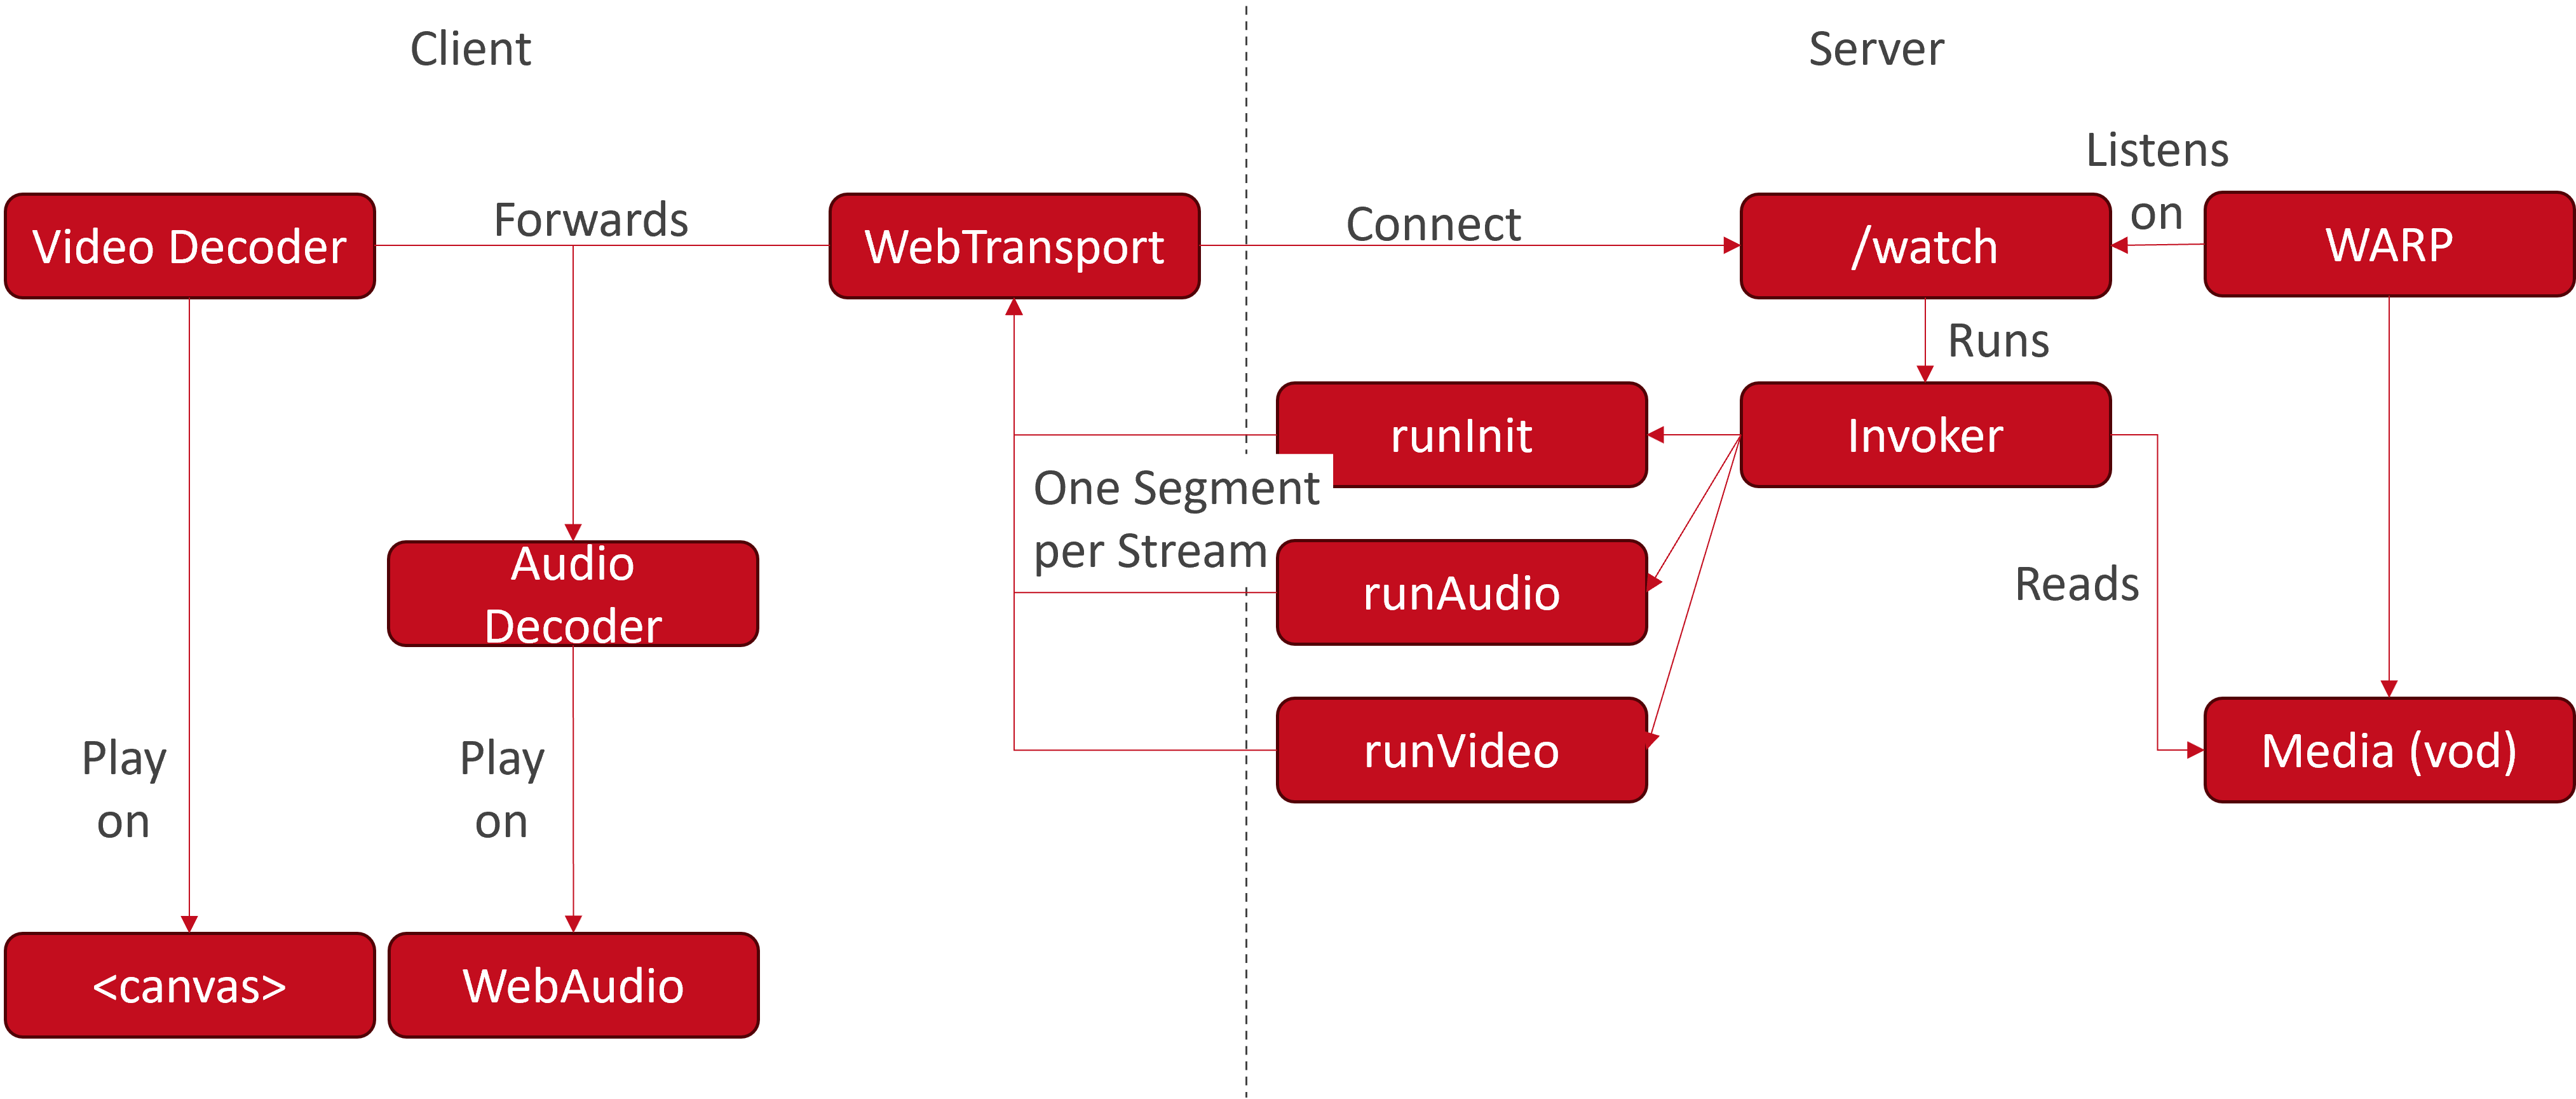
\includegraphics[width=0.49\textwidth]{images/warp.png}}
    \caption{Flow chart WARP protocol}
    \label{fig:warp}
\end{figure}

\section{Evaluation}
Over course of this project there have been several changes made to the repository of the WARP demo. The first major change was the refactoring of the server code from $webtransport-go$ to a modified version of the Rust library $quiche$. The next big change was a complete rebranding from WARP to $moq-rs$. Now the client, $moq-js$ \cite{b27} and server, $moq-rs$ \cite{b28}, code has been split up into two separate repositories. Finally, on the 1st of July the first IETF draft for the new protocol "Media Over QUIC Transport" (MOQT) \cite{b29} has been published, utilizing $moq-rs$ and defining key features of this new protocol.

Key points of MOQT include the requirement of having a producer of content, who publishes said content, as well as this content being able to consumed by a variety consumers by subscribing to the producer. Furthermore, MOQT requires to support either the QUIC network protocol directly or using WebTransport, as well as being capable to provide a wide range of different latency stages while being highly resilient without compromising scalability and driving up the cost effectiveness. Finally, it details all technical requirements for the MOQT protocol \cite{b29}.

\section{Conclusion}
In conclusion HTTP/3 and QUIC show promising results for being highly suitable to becoming the new state-of-the-art transport protocol foundation for streaming media over the network. They are offering higher security by demanding to also use the TLS encrypted HTTPS protocol without sacrificing the security for performance and latency. This lowered latency not only reduces the wait time required for a Video-on-Demand (vod) or live to start playing, but also enables more seamless real-time applications like video conferencing, live streaming and multiplayer video games. Additionally, it enables the server to send data to the client without the clients having to add to the network traffic by requesting data segments individually.

Finally, the MOQ working group has made a big step by releasing their first promising draft for MOQT based on the WARP protocol, or rather its evolution $moq-rs$.

\begin{thebibliography}{00}
\bibitem{b1} M. Nguyen, D. Lorenzi, F. Tashtarian, H. Hellwagner and C. Timmerer, "DoFP+: An HTTP/3-Based Adaptive Bitrate Approach Using Retransmission Techniques," in IEEE Access, vol. 10, pp. 109565-109579, 2022, doi: 10.1109/ACCESS.2022.3214827.
\bibitem{b2} \url{https://www.slashgear.com/netflix-is-lowering-video-bitrates-in-europe-because-of-coronavirus-19613772}
\bibitem{b3} \url{https://www.engadget.com/2020-03-20-amazon-prime-video-streaming-bitrate-europe.html}
\bibitem{b4} \url{https://en.wikipedia.org/wiki/HTTP_Live_Streaming}
\bibitem{b5} \url{https://www.iso.org/standard/57623.html}
\bibitem{b6} \url{https://w3techs.com/technologies/details/ce-httpsdefault}
\bibitem{b7} \url{https://howdoesinternetwork.com/2015/hol-head-of-line-blocking}
\bibitem{b8} \url{https://www.cloudflare.com/learning/video/what-is-mpeg-dash/}
\bibitem{b9} \url{https://en.wikipedia.org/wiki/Real-time_Transport_Protocol}
\bibitem{b10} \url{https://en.wikipedia.org/wiki/Real-Time_Messaging_Protocol}
\bibitem{b11} \url{https://datatracker.ietf.org/doc/rfc9114/}
\bibitem{b12} \url{https://developer.chrome.com/articles/webtransport/}
\bibitem{b13} \url{https://github.com/ArckyPN/tu-berlin-awt-pj-ss23-http3}
\bibitem{b14} \url{https://www.ietf.org/archive/id/draft-kpugin-rush-00.html}
\bibitem{b15} \url{https://github.com/adriancable/webtransport-go}
\bibitem{b16} \url{https://github.com/facebookexperimental/webcodecs-capture-play}
\bibitem{b17} \url{https://github.com/facebookexperimental/go-media-webtransport-server}
\bibitem{b18} \url{https://www.youtube.com/watch?v=adckQdZHECQ}
\bibitem{b19} \url{https://datatracker.ietf.org/doc/draft-jennings-mimi-quicr-proto/}
\bibitem{b20} \url{https://github.com/Quicr/qmedia}
\bibitem{b21} \url{https://github.com/Quicr/libquicr}
\bibitem{b22} \url{https://github.com/Quicr/quicrq}
\bibitem{b23} \url{https://user-images.githubusercontent.com/947528/201170693-629525d4-211e-4849-98c5-57b883bccba7.mp4}
\bibitem{b24} \url{https://user-images.githubusercontent.com/947528/181114950-400c22da-f623-4bc5-a8d6-7f4e3188a9c5.mp4}
\bibitem{b25} \url{https://datatracker.ietf.org/doc/draft-lcurley-warp/}
\bibitem{b26} \url{https://github.com/kixelated/webtransport-go}
\bibitem{b27} \url{https://github.com/kixelated/moq-js}
\bibitem{b28} \url{https://github.com/kixelated/moq-rs}
\bibitem{b29} \url{https://datatracker.ietf.org/doc/draft-ietf-moq-transport/}

\end{thebibliography}
\vspace{12pt}

\end{document}
